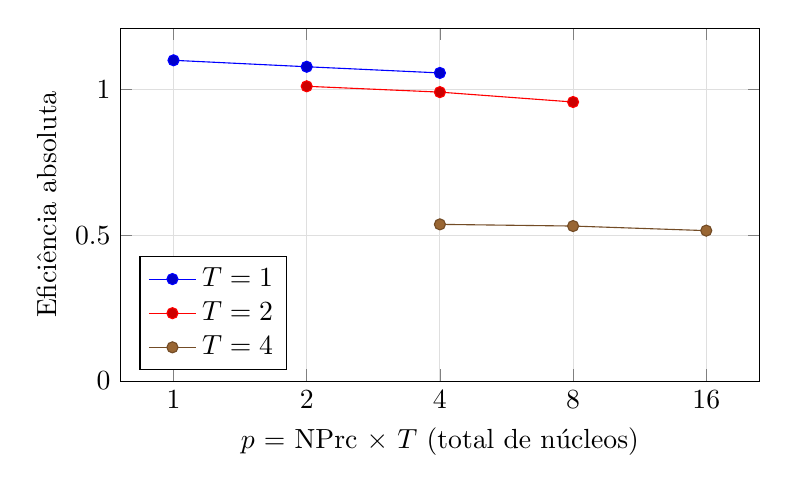
\begin{tikzpicture}
\begin{axis}[
    width=0.8\textwidth, height=0.5\textwidth,
    xmode=log, log basis x=2, ymin=0,
    xlabel={$p$ = NPrc $\times$ $T$ (total de núcleos)}, ylabel={Eficiência absoluta},
    xtick={1,2,4,8,16}, xticklabels={1,2,4,8,16},
    legend pos=south west, legend cell align=left, grid=major, grid style={gray!25},
]
\addplot+[mark=*] coordinates {(1,1.0998) (2,1.0777) (4,1.0565)};
\addlegendentry{$T=1$}
\addplot+[mark=*] coordinates {(2,1.0107) (4,0.9907) (8,0.9568)};
\addlegendentry{$T=2$}
\addplot+[mark=*] coordinates {(4,0.5373) (8,0.5315) (16,0.5158)};
\addlegendentry{$T=4$}
\end{axis}
\end{tikzpicture}
